\documentclass{beamer}
\usetheme{Madrid}
\usepackage[T1]{fontenc}
\usepackage{mathpazo}
\usepackage{graphicx}
\usepackage{booktabs}
\usepackage{tikz}
\usetikzlibrary{positioning,arrows.meta,shapes.geometric,fit,backgrounds,calc}
\definecolor{cetnavy}{RGB}{10,26,63}
\definecolor{cetlight}{RGB}{225,231,242}
\setbeamercolor{structure}{fg=cetnavy}
\setbeamercolor{frametitle}{bg=cetnavy,fg=white}
\setbeamercolor{title}{bg=cetnavy,fg=white}
\setbeamertemplate{navigation symbols}{}
% =====================================================================
%  EDIT YOUR DETAILS HERE — this ONE file feeds every abstract & deck.
%  (Change a value, recompile; all 36 documents update.)
% =====================================================================
\newcommand{\seminarName}{Aflah Muhammed P}      % <-- your full name (guessed from your email; please verify)
\newcommand{\seminarRoll}{TVE00CS000}            % <-- your university register/roll number
\newcommand{\seminarClassRoll}{00}               % <-- your class roll no (the short one)
\newcommand{\seminarGuide}{Prof.\ <Guide Name>}  % <-- your guide
\newcommand{\seminarDept}{Department of Computer Science and Engineering}
\newcommand{\seminarCollege}{College of Engineering Trivandrum}
\newcommand{\seminarShortCollege}{CET}           % shown in the slide footer, e.g. "Aflah Muhammed P (CET)"
\newcommand{\seminarShortTitle}{B.Tech Seminar}  % middle of the slide footer
\newcommand{\seminarDate}{July 31, 2026}
% ---------------------------------------------------------------------
% Optional: put a logo image named  cet_logo.png  in this folder and it
% will appear on every title slide automatically. If absent, it is skipped.
% =====================================================================

\title[\seminarShortTitle]{Design Patterns for Securing LLM Agents against Prompt Injection}
\author[\seminarName\ (\seminarShortCollege)]{\seminarName \\ \seminarRoll \\ Roll No: \seminarClassRoll \\ Guide: \seminarGuide}
\institute[\seminarShortCollege]{\seminarDept \\ \seminarCollege}
\date{\seminarDate}
\titlegraphic{\IfFileExists{cet_logo.png}{\includegraphics[height=1.1cm]{cet_logo.png}}{}}
\begin{document}
\begin{frame}\titlepage\end{frame}
\begin{frame}{Table of Contents}\tableofcontents\end{frame}
\section{Introduction}
\begin{frame}{What Are LLM Agents?}
\textbf{\textit{From chatbots to actors}}
\begin{itemize}
\item LLMs now call tools, read files, and query APIs.
\item Agents plan, retrieve, and act autonomously.
\item Utility comes from consuming external, untrusted content.
\item That same content becomes a new attack surface.
\end{itemize}
\end{frame}

\begin{frame}{Prompt Injection in One Slide}
\begin{itemize}
\item Malicious instructions hidden inside ingested data.
\item Natural-language analogue of SQL injection.
\item Model cannot separate trusted commands from data.
\item Result: data exfiltration, unauthorized actions, corrupted output.
\end{itemize}
\end{frame}

\section{Literature Survey}
\begin{frame}{Prior Defenses and Their Limits}
\textbf{\textit{Mostly probabilistic mitigations}}
\begin{itemize}
\item Prompt engineering and delimiters -- easily bypassed.
\item Adversarial fine-tuning -- no guarantee, broken adaptively.
\item Learned injection detectors -- false negatives remain.
\item Benchmarks (AgentDojo) expose fragility of heuristics.
\end{itemize}
\end{frame}

\begin{frame}{Toward Security by Design}
\begin{itemize}
\item CaMeL: control/data-flow separation for agents.
\item Dual-LLM idea popularized for quarantining untrusted text.
\item Borrows from control-flow integrity and access control.
\item This paper unifies such ideas into reusable patterns.
\end{itemize}
\end{frame}

\section{Motivation}
\begin{frame}{Why Heuristic Defenses Are Not Enough}
\begin{itemize}
\item Any single successful injection can be catastrophic.
\item Attackers adapt faster than filters improve.
\item Security cannot rely on model ``willpower''.
\item Need guarantees independent of the underlying model.
\end{itemize}
\end{frame}

\section{Problem Statement}
\begin{frame}{The Precise Problem}
\begin{itemize}
\item Agents must process attacker-controllable inputs.
\item Threat model: files, emails, calendars, reviews, resumes, APIs.
\item Goal: untrusted input must not cause consequential actions.
\item Achieve this without destroying agent usefulness.
\end{itemize}
\end{frame}

\section{Objectives}
\begin{frame}{Goals and Contributions}
\textbf{\textit{A principled toolkit}}
\begin{itemize}
\item State one core containment principle.
\item Catalog six reusable secure design patterns.
\item Characterize each pattern's security-utility trade-off.
\item Ground patterns in ten real application case studies.
\end{itemize}
\end{frame}

\section{Methodology Overview}
\begin{frame}{The Core Design Principle}
\begin{center}
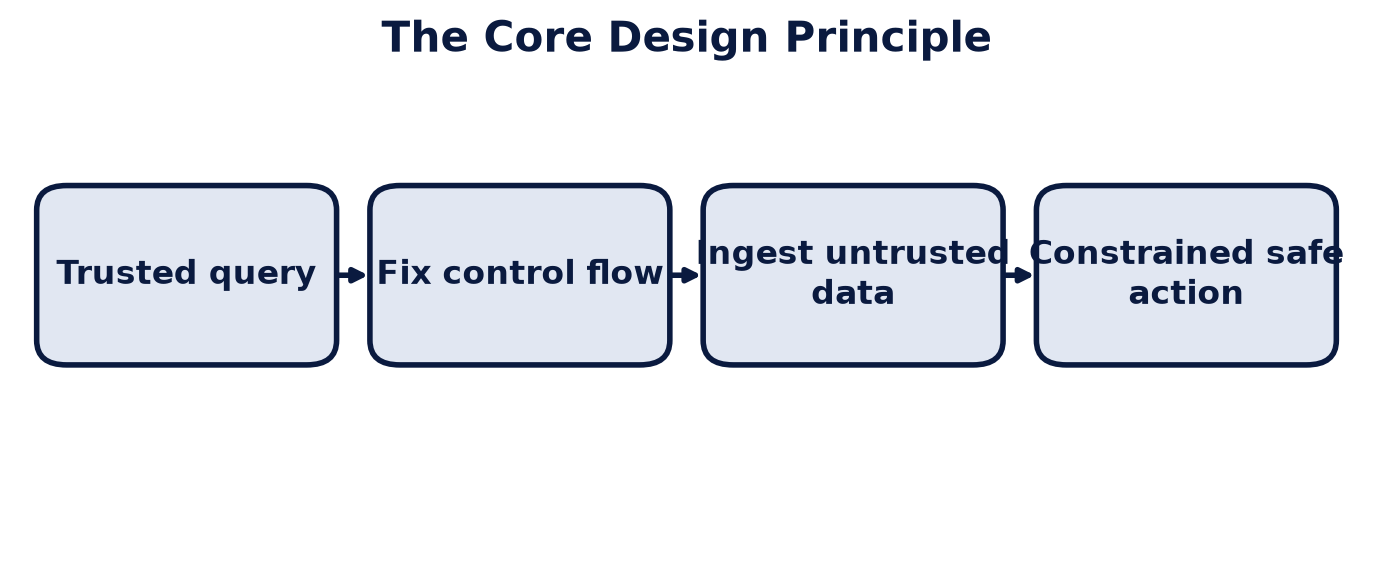
\includegraphics[width=0.9\textwidth,height=0.62\textheight,keepaspectratio]{images/designpatterns_1.png}
\end{center}
\begin{itemize}
\item After ingesting untrusted input, consequential actions are blocked.
\item Control flow is decided \emph{before} seeing untrusted data.
\end{itemize}
\end{frame}

\section{System Architecture}
\begin{frame}{Dual-LLM Pattern Architecture}
\begin{center}
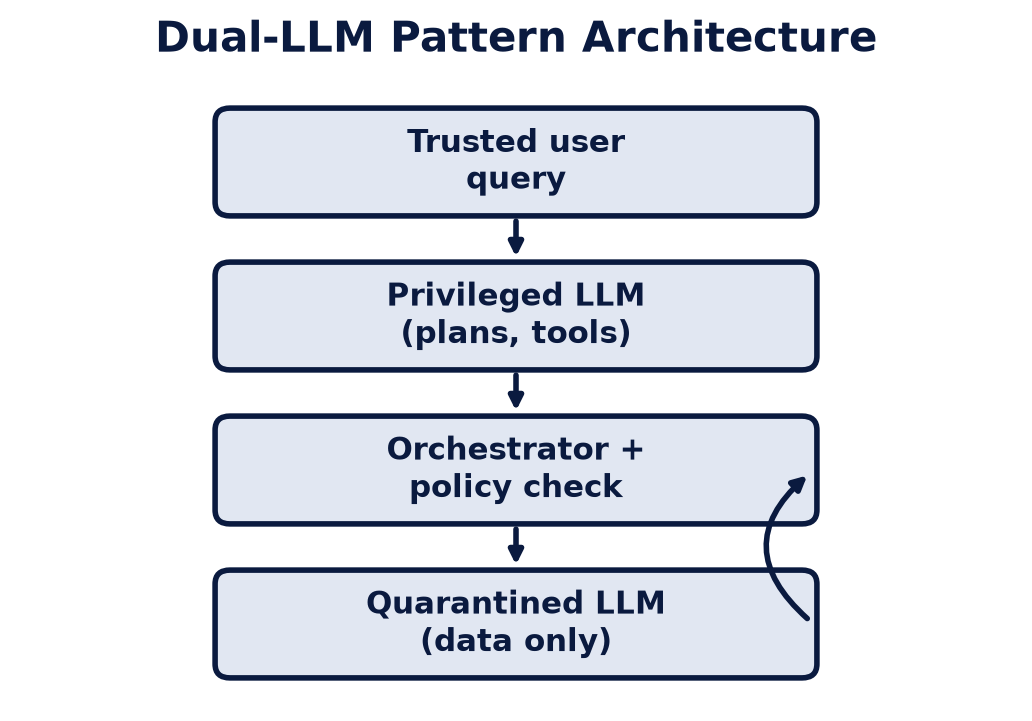
\includegraphics[width=0.9\textwidth,height=0.62\textheight,keepaspectratio]{images/designpatterns_2.png}
\end{center}
\begin{itemize}
\item Privileged LLM never reads raw untrusted text.
\item Quarantined LLM returns only symbolic references.
\end{itemize}
\end{frame}

\section{Data Collection}
\begin{frame}{Case Studies as Evaluation Scope}
\textbf{\textit{Ten application scenarios}}
\begin{itemize}
\item OS assistant, SQL agent, email/calendar assistant.
\item Customer-service and booking chatbots.
\item Product recommender, resume screening assistant.
\item Medication and diagnosis chatbots, coding agent.
\end{itemize}
\end{frame}

\section{Model Development}
\begin{frame}{The Containment Decision}
\begin{center}
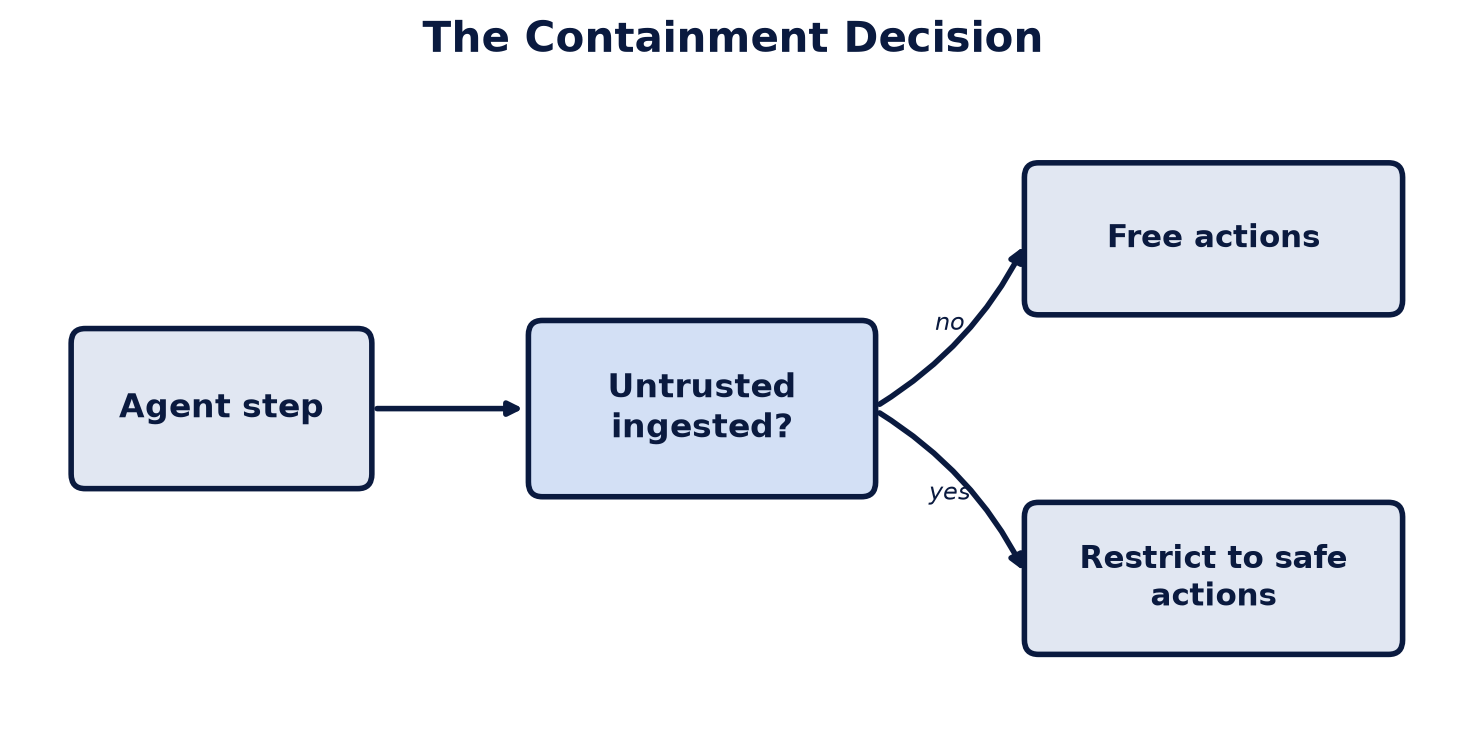
\includegraphics[width=0.9\textwidth,height=0.62\textheight,keepaspectratio]{images/designpatterns_3.png}
\end{center}
\end{frame}

\begin{frame}{The Six Design Patterns}
\begin{itemize}
\item \textbf{Action-selector:} NL mapped to fixed tool calls.
\item \textbf{Plan-then-execute:} commit action sequence before data.
\item \textbf{LLM map-reduce:} isolated instances per data item.
\item \textbf{Dual LLM:} privileged planner, quarantined reader.
\item \textbf{Code-then-execute:} generate a program, then run it.
\item \textbf{Context-minimization:} drop prompt after selecting actions.
\end{itemize}
\end{frame}

\section{Results}
\begin{frame}{Security vs. Utility Trade-off}
\begin{center}
\footnotesize
\begin{tabular}{@{}lll@{}}
\toprule
\textbf{Pattern} & \textbf{Guarantee} & \textbf{Utility limit} \\
\midrule
Action-selector & No injection feedback & Hardcoded ops only \\
Plan-then-execute & Control-flow integrity & Params still influenced \\
LLM map-reduce & No cross-item spread & Per-item errors \\
Dual LLM & Strict isolation & Constrained outputs \\
Code-then-execute & Explicit data flow & Params vulnerable \\
Context-minimization & Blocks user-prompt inject. & Narrow scope \\
\bottomrule
\end{tabular}
\end{center}
\begin{itemize}
\item Stronger containment generally means less flexibility.
\item CaMeL (code-then-execute) shows provable security is achievable.
\end{itemize}
\end{frame}

\section{Discussions}
\begin{frame}{Why the Patterns Work}
\begin{itemize}
\item Guarantees come from architecture, not model behavior.
\item Untrusted data loses power over consequential actions.
\item Patterns compose; agents mix them per subtask.
\item Trade-off is explicit and can be chosen deliberately.
\end{itemize}
\end{frame}

\section{Challenges}
\begin{frame}{Limitations and Open Problems}
\begin{itemize}
\item Some patterns sharply reduce agent flexibility.
\item Parameters of actions can still carry injected data.
\item Defining ``consequential action'' is application-specific.
\item No single pattern fits every use case.
\end{itemize}
\end{frame}

\section{Future Work}
\begin{frame}{Directions Ahead}
\begin{itemize}
\item Automated policy synthesis for tool permissions.
\item Better data-provenance and information-flow tracking.
\item Hybrid patterns balancing security and utility.
\item Standard benchmarks for provable-security defenses.
\end{itemize}
\end{frame}

\section{Conclusion}
\begin{frame}{Takeaways}
\begin{itemize}
\item Prompt injection needs design-level, not heuristic, defenses.
\item One principle: contain actions after untrusted ingestion.
\item Six patterns give provable resistance with clear trade-offs.
\item Security by construction is practical for real agents.
\end{itemize}
\end{frame}

\section{References}
\begin{frame}{References}
\footnotesize
\begin{itemize}
\item L. Beurer-Kellner et al., ``Design Patterns for Securing LLM Agents against Prompt Injections,'' arXiv:2506.08837, 2025.
\item E. Debenedetti et al., ``Defeating Prompt Injections by Design (CaMeL),'' arXiv:2503.18813, 2025.
\item E. Debenedetti et al., ``AgentDojo: A Dynamic Environment to Evaluate Prompt Injection Attacks and Defenses for LLM Agents,'' NeurIPS, 2024.
\end{itemize}
\end{frame}
\begin{frame}\vfill\centering{\Huge Thank You}\vfill\end{frame}
\end{document}
